\documentclass[10pt,letterpaper]{article}
\usepackage{amsmath,amsthm,amsfonts,amssymb,amscd}
\usepackage{fullpage}
\usepackage{lastpage}
\usepackage{enumerate}
\usepackage{fancyhdr}
\usepackage{mathrsfs}
\usepackage[framed]{mcode}
\usepackage{xcolor}
\usepackage{dsfont}
\usepackage{gensymb}
\usepackage{graphicx}
\usepackage[margin=3cm]{geometry}
\setlength{\parindent}{0.0in}
\setlength{\parskip}{0.05in}

% Edit these as appropriate
\newcommand\course{CIS580}
\newcommand\semester{Spring 2015}     % <-- current semester
\newcommand\hwnum{}                  % <-- homework number
\newcommand\yourname{Michael O'Meara and Michael Woods} % <-- your name
\newcommand\hwdate{Due: May 6, 2015}           % <-- HW due date

\newenvironment{answer}[1]{
  \subsubsection*{1}
}


\pagestyle{fancyplain}
\headheight 20pt
\lhead{\yourname\ \login\\\course\ --- \semester}
\chead{\textbf{\Large Project 2 Final Report \hwnum}}
\rhead{\hwdate}
\headsep 10pt

\begin{document}

\begin{enumerate}[]

\item \textbf{After RANSAC}

\begin{figure}[h!]
 \center
  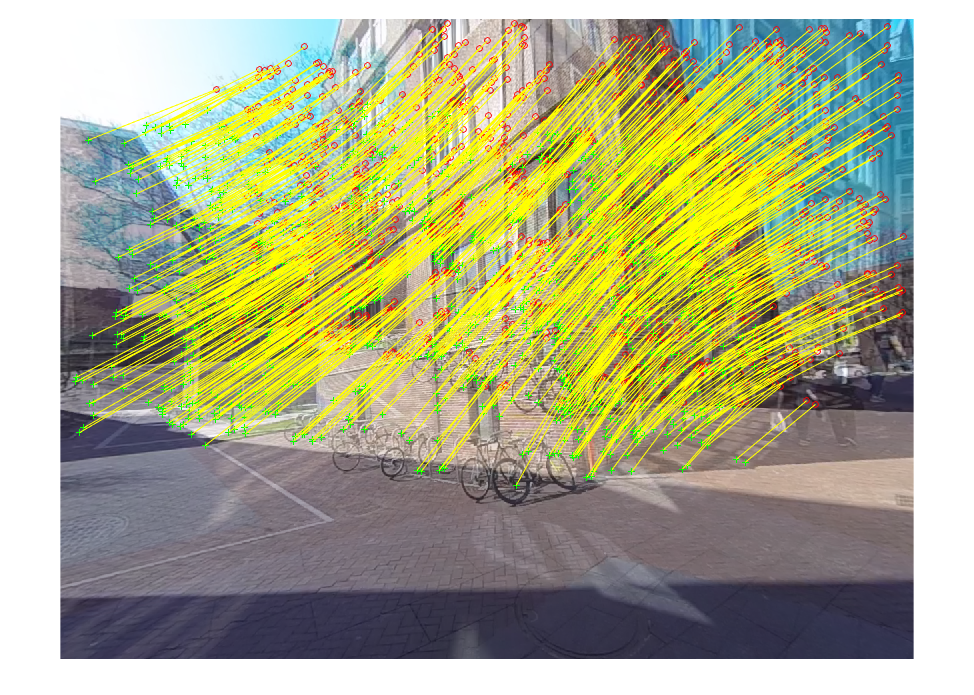
\includegraphics[width=5in]{../images/after_ransac1-2}
  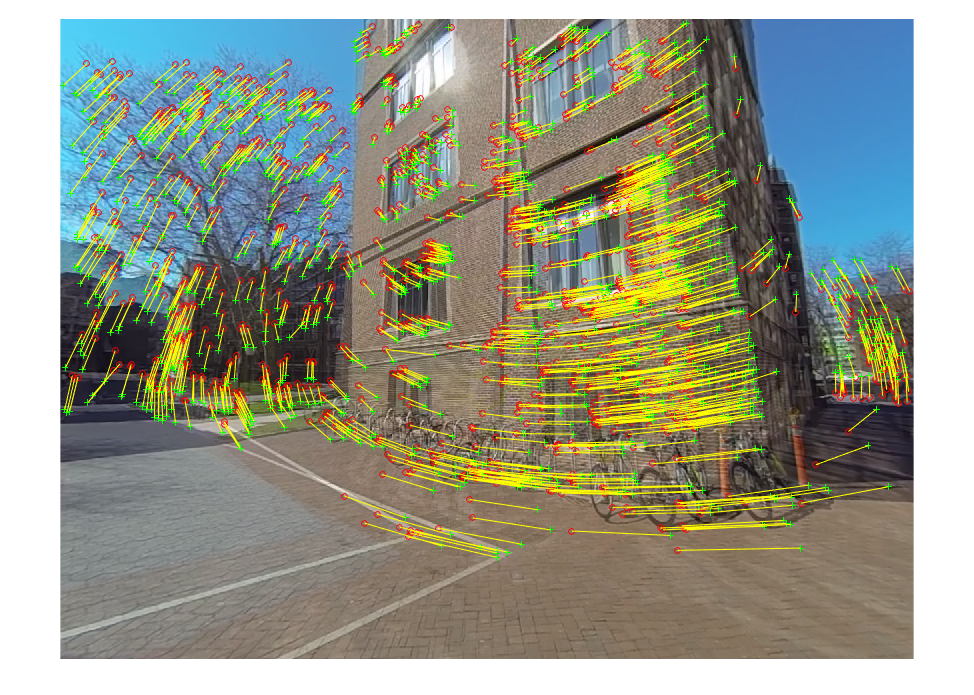
\includegraphics[width=5in]{../images/after_ransac5-6}
  \caption
   {Matches between images [1,4] and [5,6]}
\end{figure} \\

\newpage

\item
\begin{eqnarray*}
F &=&
\begin{bmatrix}
      1.83625947723393e-06   &  -2.51716925025149e-05   &    0.00954074607953851 \\
      2.77336539369028e-05   &  -8.0892063262401e-07   &   -0.00245769694374222 \\
       -0.0140295140445968    &   0.00103929740763176     &    0.999852501661995 \\
\end{bmatrix}
\end{eqnarray*}

The number of Inliers between images 1 and 4 was 417 out of 470 matches. \\

\item 
\begin{eqnarray*}
E &=&
\begin{bmatrix}
        0.0545907724488276    &    -0.673097985417172      &  -0.0563146312113391 \\
        0.725124089635866      &    -0.0327622911205873    &   0.687130575186785 \\
        0.0258863359957035    &    -0.729705929390185      & -0.0928440933910298 \\
\end{bmatrix} \\
Cset\{1\} &=&
\begin{bmatrix}
        -0.735382629589736 \\
        0.0311971080993757 \\
         0.676933621962981 \\
\end{bmatrix} \\
Rset\{1\} &=&
\begin{bmatrix}
        0.0143917426481273      &   0.084523963272568    &    -0.996317508315621 \\
        0.0345906392414555      &  -0.995866373697126    &    -0.083986031077812 \\
        -0.999297936263464       & -0.033254554154782     &  -0.0172559904829925 \\
\end{bmatrix} \\
Cset\{2\} &=&
\begin{bmatrix}
         0.735382629589736 \\
       -0.0311971080993757 \\
        -0.676933621962981 \\
\end{bmatrix} \\
Rset\{2\} &=&
\begin{bmatrix}
        0.0143917426481273     &    0.084523963272568    &    -0.996317508315621 \\
        0.0345906392414555      &  -0.995866373697126   &     -0.083986031077812 \\
        -0.999297936263464      &  -0.033254554154782    &   -0.0172559904829925 \\
\end{bmatrix} \\
Cset\{3\} &=&
\begin{bmatrix}
        -0.735382629589736 \\
        0.0311971080993757 \\
         0.676933621962981 \\
\end{bmatrix} \\
Rset\{3\} &=&
\begin{bmatrix}
         0.994498337743052    &    0.0856976000083201    &   -0.0602409958344102 \\
       -0.0773907430675559  &       0.988645071076093    &     0.128808370552532 \\
        0.0705955318257396   &     -0.123437614971129    &     0.989838080746786 \\
\end{bmatrix} \\
Cset\{4\} &=&
\begin{bmatrix}
         0.735382629589736 \\
       -0.0311971080993757 \\
        -0.676933621962981 \\
\end{bmatrix} \\
Rset\{4\} &=&
\begin{bmatrix}
         0.994498337743052     &   0.0856976000083201    &   -0.0602409958344102 \\
       -0.0773907430675559    &     0.988645071076093     &    0.128808370552532 \\
        0.0705955318257396     &   -0.123437614971129     &    0.989838080746786 \\
\end{bmatrix}
\end{eqnarray*}

\newpage 

\item PnPRANSAC results for images 2,3,5,6

\begin{eqnarray*}

\\ inliers for image 2: 123 / 202 \\

C &=& 
\begin{bmatrix}
-0.12335768 \\
-0.02667446 \\
0.12635737   
\end{bmatrix} \\ 
R &=& 
\begin{bmatrix}
0.97443115 & 0.05954343 & -0.21665296 \\
-0.02380564 & 0.98617886 & 0.16396509 \\
0.22342161 & -0.15461513 & 0.96238087   
\end{bmatrix} \\

\\inliers for image 3: 185 / 725 \\
C &=& 
\begin{bmatrix}
-0.29259455 \\
0.03978676 \\
0.14606147   
\end{bmatrix} \\ 
R &=& 
\begin{bmatrix}
0.99900499 & 0.03949060 & -0.02072474 \\
-0.03556627 & 0.98581380 & 0.16403106 \\
0.02690842 & -0.16313075 & 0.98623744   
\end{bmatrix} \\

\\inliers for image 5: 44 / 422 \\
C &=& 
\begin{bmatrix}
-0.40883437 \\
-0.00584841 \\
0.41703507   
\end{bmatrix} \\ 
R &=& 
\begin{bmatrix}
0.96745992 & -0.01983794 & -0.25224544 \\
0.05316520 & 0.99060423 & 0.12600286 \\
0.24737576 & -0.13531340 & 0.95942458   
\end{bmatrix} \\

\\ inliers for image 6: 24 / 659 \\
C &=& 
\begin{bmatrix}
-0.41548468 \\
-0.03244642 \\
0.40228481   
\end{bmatrix} \\ 
R &=& 
\begin{bmatrix}
0.96975839 & 0.08004649 & -0.23056717 \\
-0.04697035 & 0.98823782 & 0.14553279 \\
0.23950459 & -0.13030182 & 0.96211173   
\end{bmatrix} \\

\end{eqnarray*}

\item

\begin{figure}[h!]
 \center
  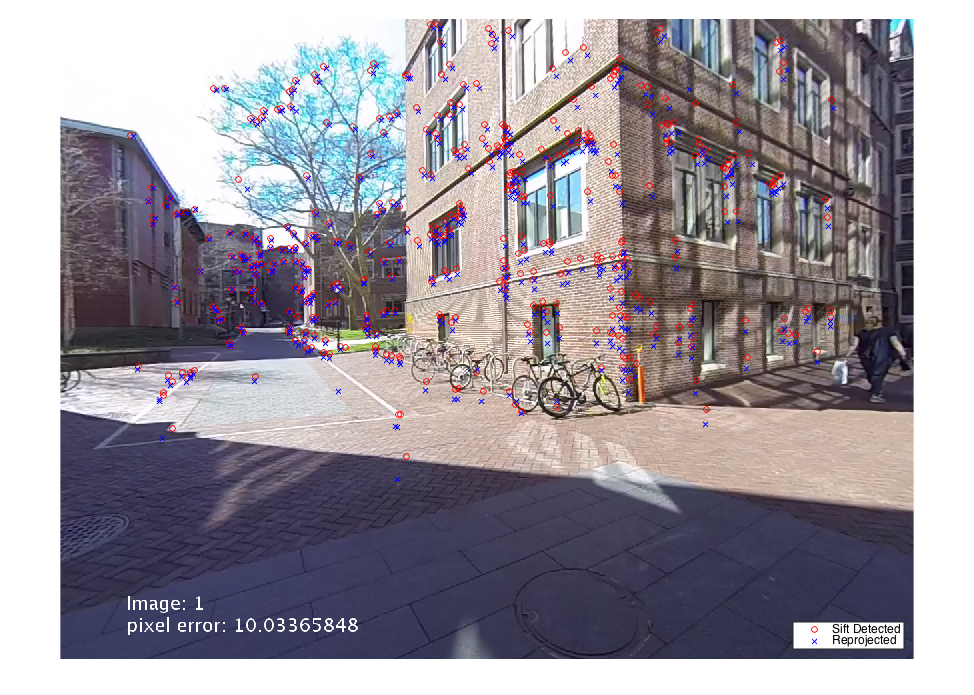
\includegraphics[width=5in]{../images/2D-triangulation-img1}
  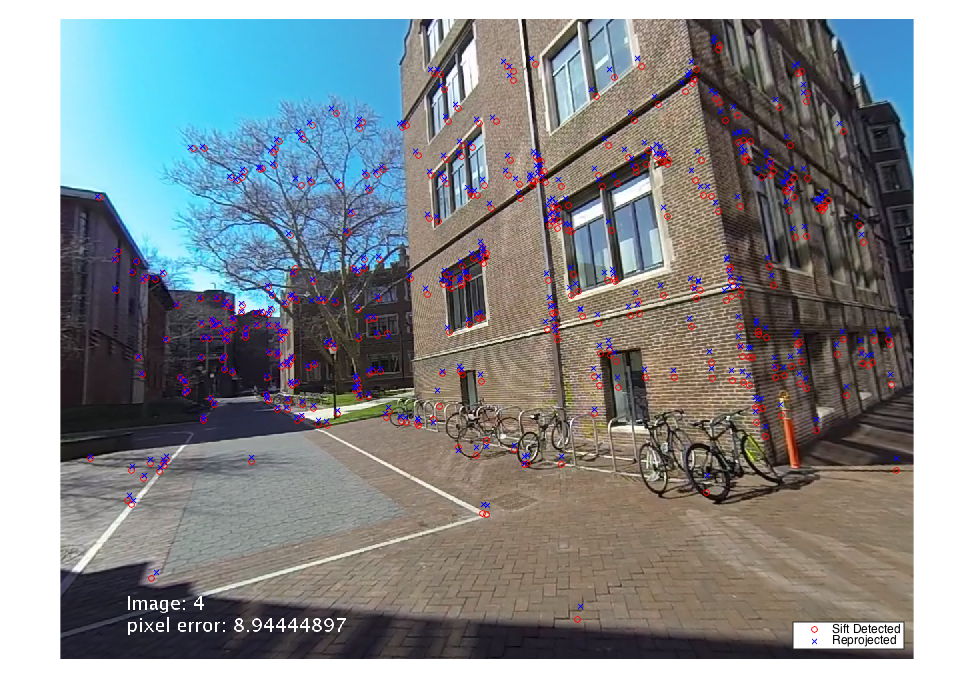
\includegraphics[width=5in]{../images/2D-triangulation-img4}
  \caption
   {}
\end{figure} \\

\begin{figure}[h!]
 \center
  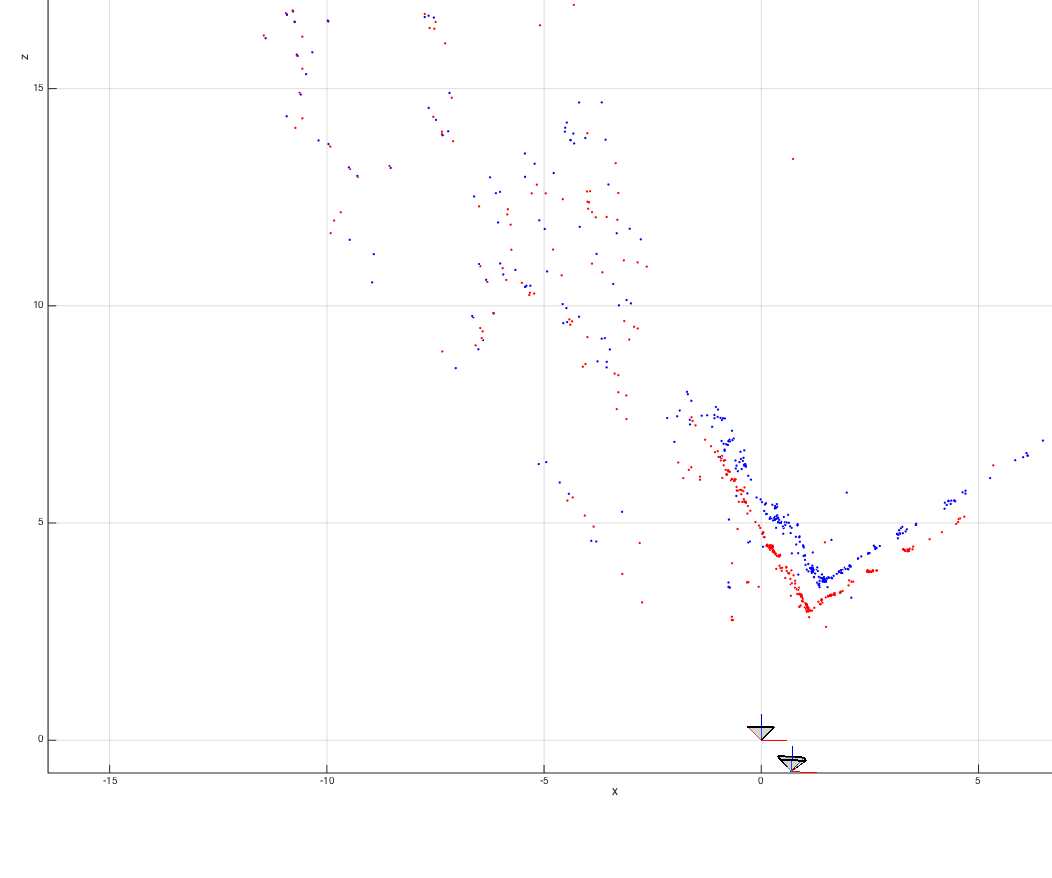
\includegraphics[width=5in]{../images/3D_linear_nonlinear_triangulation}
  \caption
   {Linear vs NonLinear Triangulation}
\end{figure} \\

\item 
\begin{figure}[h!]
 \center
  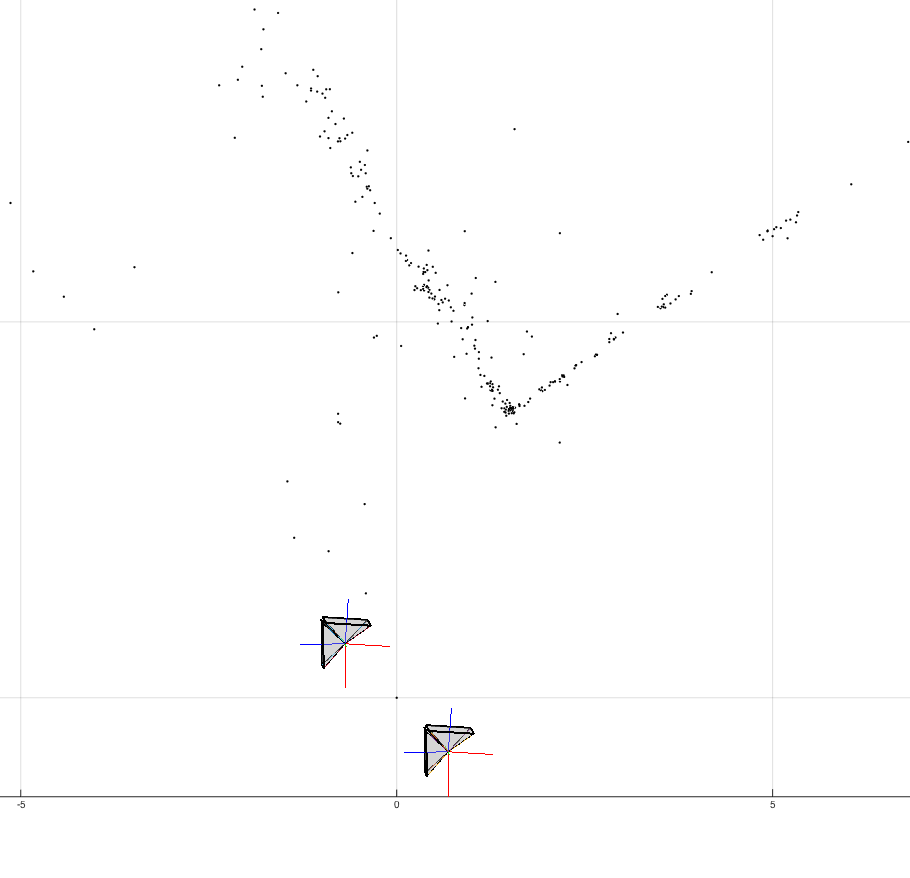
\includegraphics[width=5in]{../images/camera_poses}
  \caption
   {Camera poses, only one is good}
\end{figure} \\


\newpage

\begin{figure}[h!]
 \center
  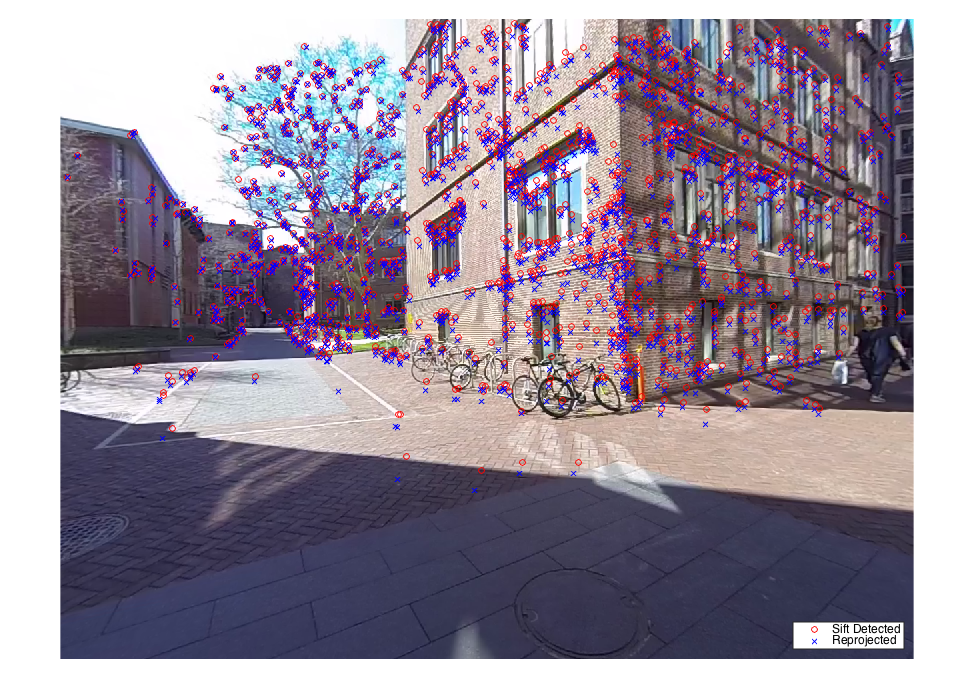
\includegraphics[width=5in]{../images/final-img1}
  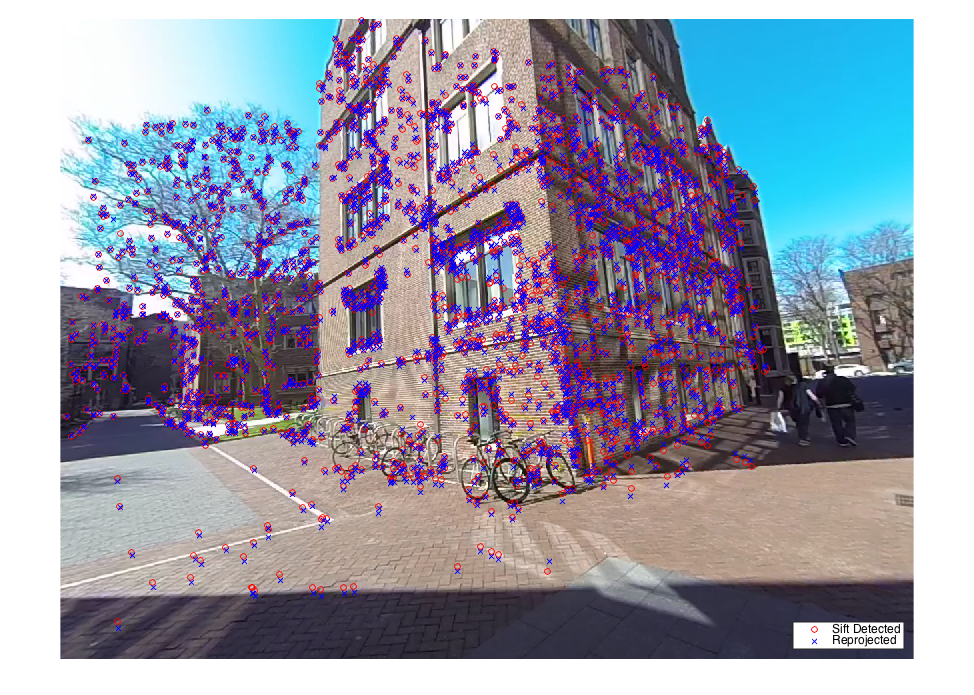
\includegraphics[width=5in]{../images/final-img2}
  \caption
   {3D projections to 2D points}
\end{figure} \\

\begin{figure}[h!]
 \center
  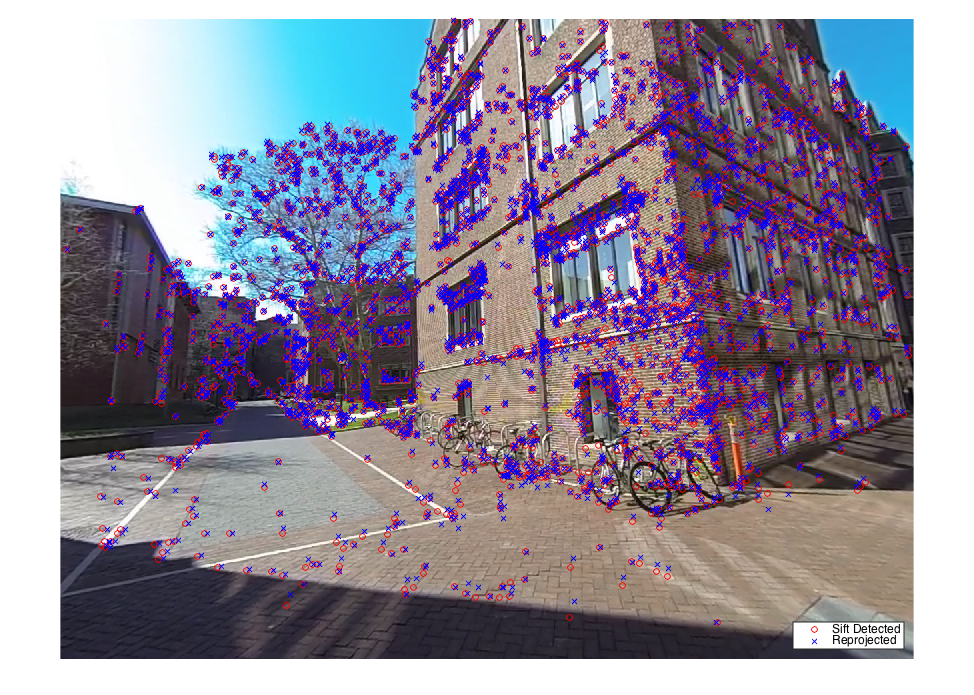
\includegraphics[width=5in]{../images/final-img3}
  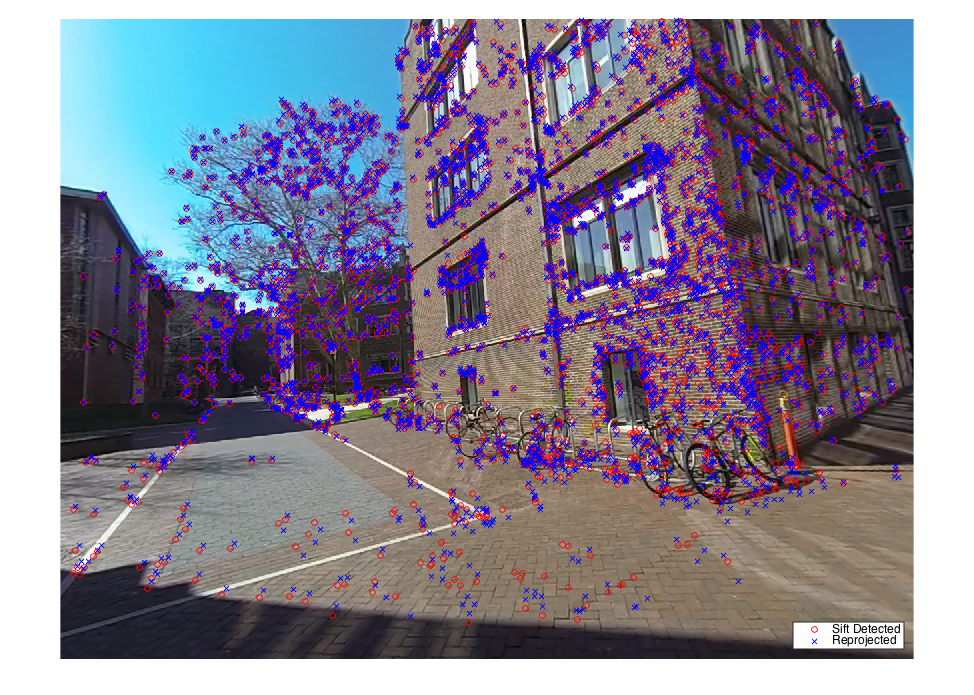
\includegraphics[width=5in]{../images/final-img4}
  \caption
  {3D projections to 2D points}
\end{figure} \\

\begin{figure}[h!]
 \center
  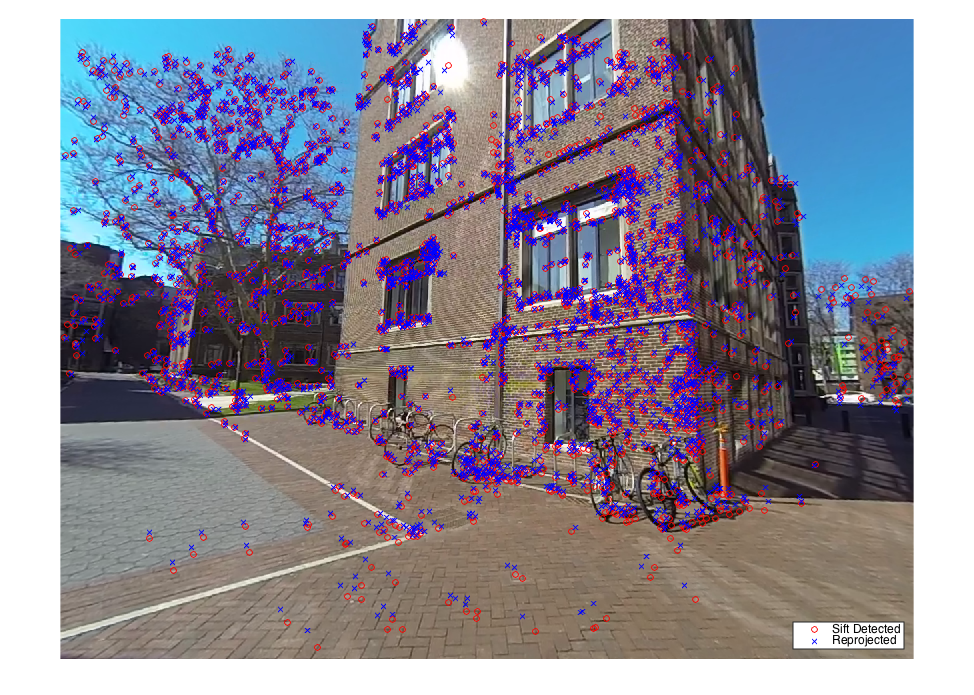
\includegraphics[width=5in]{../images/final-img5}
  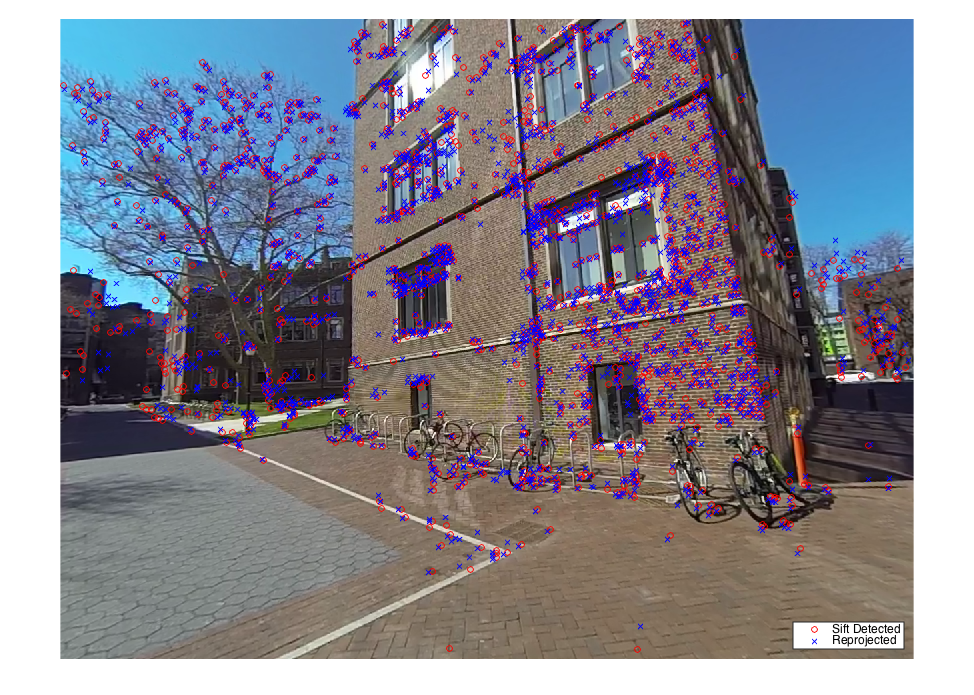
\includegraphics[width=5in]{../images/final-img6}
  \caption
   {3D projections to 2D points}
\end{figure} \\

\begin{figure}[h!]
 \center
  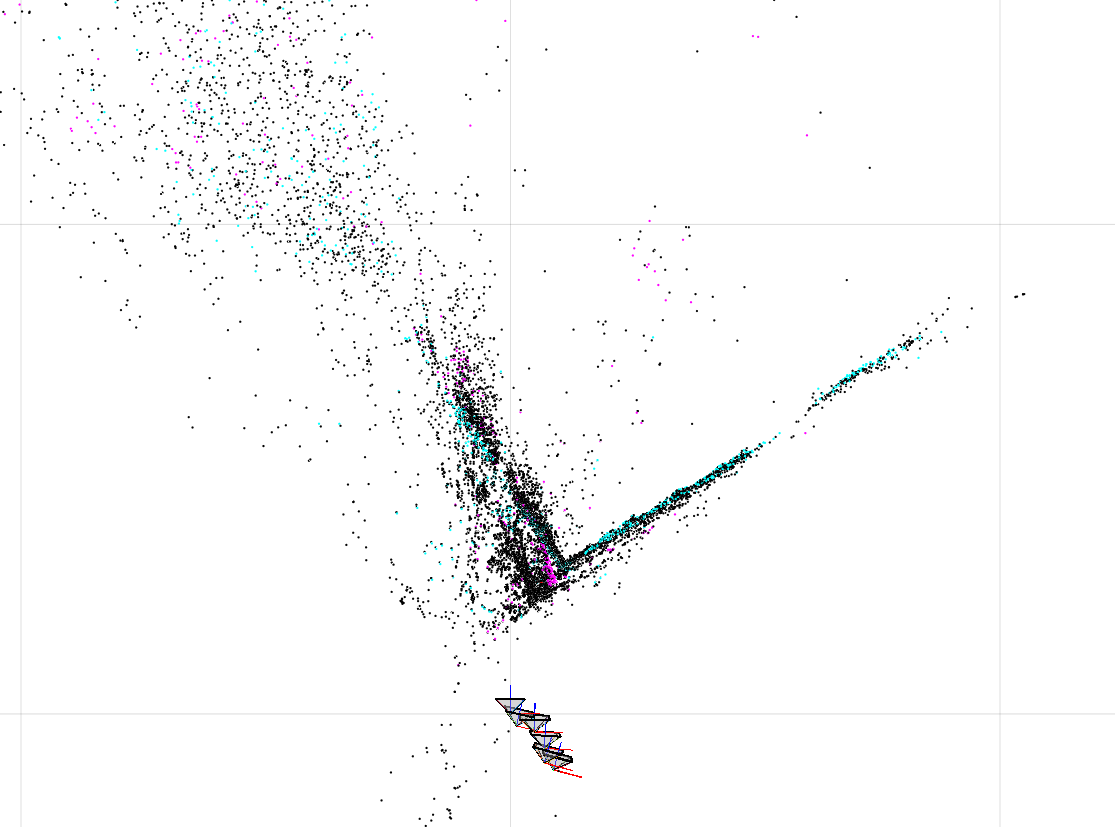
\includegraphics[width=5in]{../images/diff_colors_per_iteration_3D}
  \caption
   {Adding new point with different colors}
\end{figure} \\

\begin{figure}[h!]
 \center
  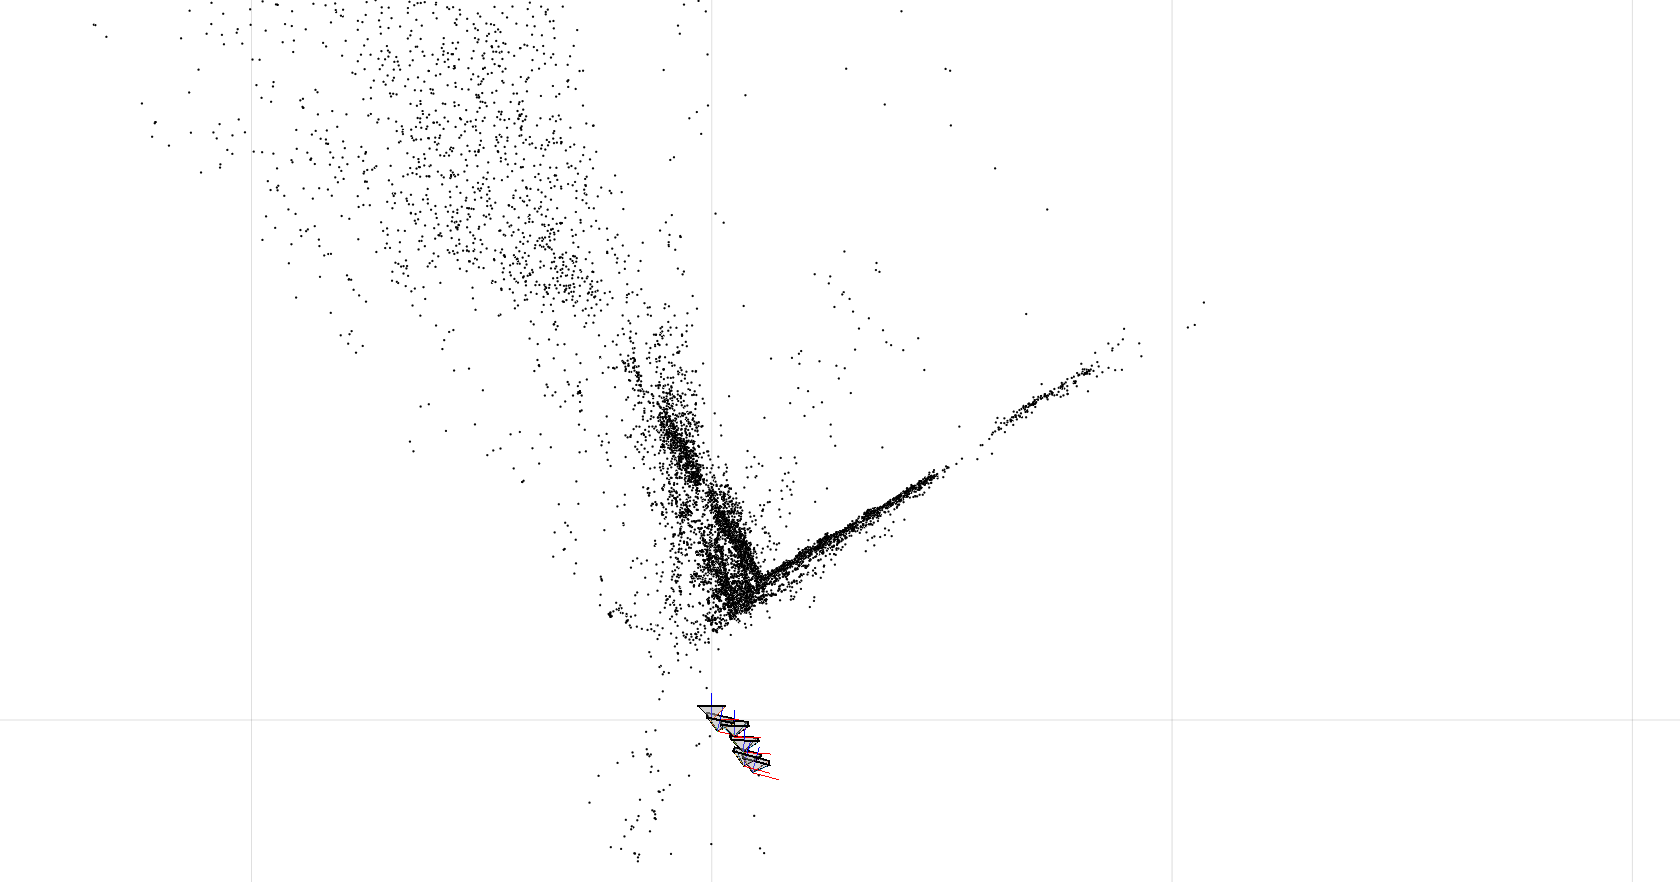
\includegraphics[width=5in]{../images/final-3d-top}
  \caption
   {3D top view}
\end{figure} \\
\begin{figure}[h!]
 \center
  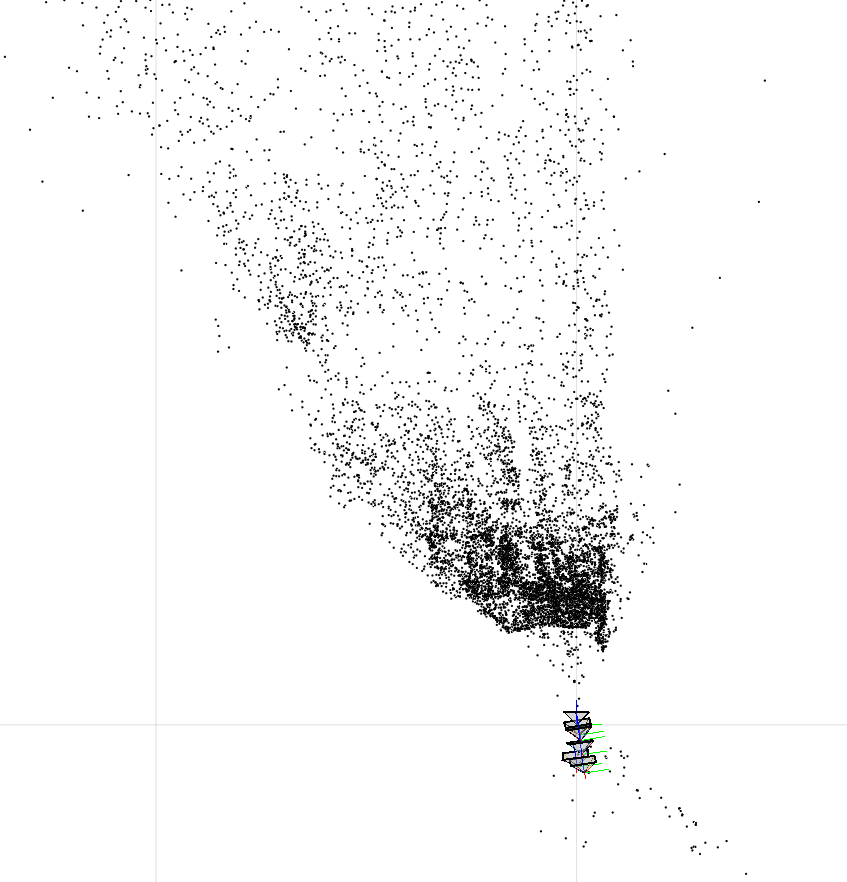
\includegraphics[width=5in]{../images/final-3d-side}
  \caption
   {3D side view}
\end{figure} \\
\begin{figure}[h!]
 \center
  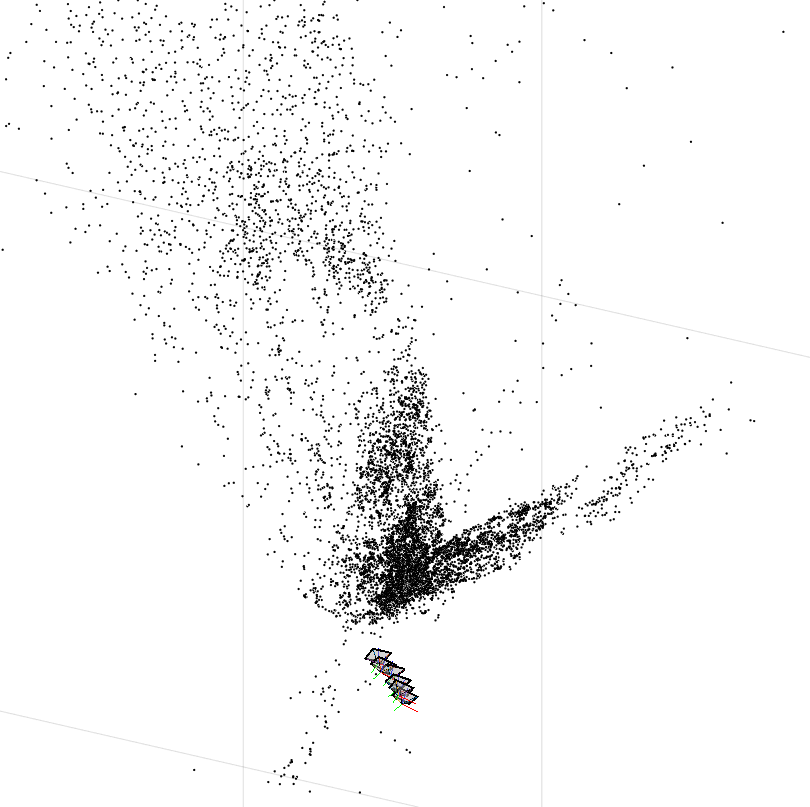
\includegraphics[width=5in]{../images/final-3d-oblique}
  \caption
   {3D oblique view}
\end{figure} \\

\newpage




\end{enumerate}
\end{document}
